\documentclass[document.tex]{subfiles}
\begin{document}

\chapter {Background}
\label {ch:background}

\todo {Add an overview of this section}

\sectionnote {AC}
\section {Workflow Framework Types and Notation}
\label {sec:overview-of-workflows}

A workflow framework is an implementation of a workflow notation into software which can be used by a developer to create and manage a workflow for their system. The framework will keep track of the state of the workflow and all of the guard conditions on the transitions. This lowers the complexity of the system as the workflow can be abstracted from the implementation of the rest of the system. This abstraction allows transitions and new activities to be added easily without modifying the rest of the system.

There are two common notations used to describe workflows: state based and Business Process Model Notation (BPMN) \cite{bpmn}. State based workflows are implemented in software using the idea of a state machine where each state is a step in the workflow. BPMN based workflows are implemented in software using the idea of a flowchart where each process is a step in the workflow. Each notation has its own strengths and weaknesses and both can be implemented in software to handle all types of workflows.

State based workflows are very good at non-linear looping workflows. The state based model assumes that a workflow is only ever in a single state which makes workflows designed using this notation robust. However, due to the single state limitation the state based model is a poor choice for modeling workflows with parallel activities. In order to model parallel activities a state must be composed of multiple individual state machines. Each of these state machines must implement guard conditions and communicate with each other in order to stay synchronized. Figure \ref{fig:state-machine-example-diagram} provides an example of a state machine. The details of the state machine are covered in section \ref{sec:stonepath-prototyping-results}.

\begin{figure}[!ht]
\centering \includegraphics[height=5in]{./img/prototypes/stonepath-state-machine}
\caption{State machine example of a simple issue tracking system}
\label{fig:state-machine-example-diagram}
\end{figure}

\FloatBarrier

Unlike the state based model, BPMN is well suited to non-looping parallel workflows. BPMN allows multiple processes to be executed concurrently by branching  control flow and merging it back together at some later time. The major downside to this branching method is that looping can become very complicated and unstable when multiple control flows exist. Figure \ref{fig:bpmn-example-diagram} displays the BMPN diagram of a simple issue tracking system which is covered in detail in section \ref{sec:ruote-prototyping-results}.

\begin{figure}[!ht]
\centering 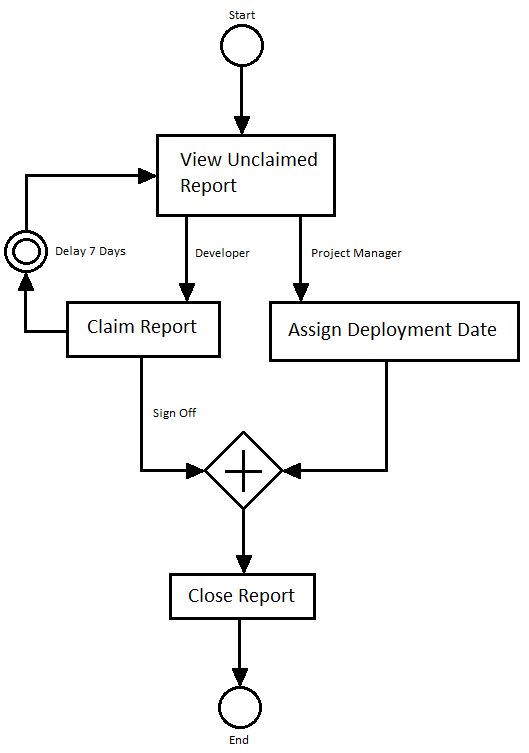
\includegraphics[height=5in]{./img/prototypes/ruote-bpmn-diagram}
\caption{BPMN example of a simple issue tracking system.}
\label{fig:bpmn-example-diagram}
\end{figure}

\FloatBarrier

Another feature of BPMN that cannot be modelled using state based modelling is the ability to express responsibility and assignment of work for individual processes. This concept of a 'role' is used by any workflow involving more than one group that perform different actions during each process. For example, a software project with the roles of developer, manager, and tester each have different tasks during each step of a project. While this can be implemented in software to work with a state based model state based diagrams cannot express the idea of a role.

\sectionnote {BM}
\section {Ruby on Rails}

Ruby on Rails \cite{rails} (often called ``Rails'') is a web application framework built on the Ruby programming language. It uses Ruby's dynamic nature and flexible syntax to provide a set of domain-specific languages (DSLs) for specific programming tasks, such as defining how objects are saved to relational databases.

Though Rails is often called a ``model-view-controller'' (MVC) web framework, its flavor of MVC differs from the conventional definition. ``Model'' refers specifically to a class of object that can be persisted to a database using Rails' object-relational mapper (ORM), ActiveRecord. Though domain logic often is encoded in models, it may also be extracted to separate service classes which perform actions that impact multiple model instances at once.

Rails' views and controllers are somewhat more conventional. Views are templates written in a domain specific language (such as ERB \cite{erb} or Haml \cite{haml}) that generates output in a specific format, often HTML. Controllers produce HTTP responses in response to HTTP requests to specific URLs. Often, each controller class corresponds to a specific model class, and each method therein (also known as an \emph{action}) is associated with a logical operation, such as ``delete the instance of the model specified by the ID in the URL.'' Each action is usually associated with a specific view. The precise mappings from HTTP requests to controllers and actions are provided by \emph{routes}, which are specified in another DSL.

%The concept of \emph{convention over configuration} pervades Rails %\cite{rails-article}. Convention over configuration means that common design %decisions are made by the framework itself, instead of requiring the developer %to make them themselves; for example, controller actions will by default render %a view of the same name. This policy is an ingrained part of the Rails %community; any new library (such as a new workflow platform) must follow it in %order to be accepted.

As this report includes sample code that Rails models and controllers, Figure \ref{fig:background-rails-code} provides an example of a model and controller, along with a few notes on the composition of each.

\begin{figure}[!ht]
  \begin{lstlisting}
# In app/models/order.rb:
class Order < ActiveRecord::Base
  belongs_to :buyer  # An order has a foreign key to one buyer
  has_many :items    # Zero or more items have foreign keys to an order

  # ...
end

# In app/controllers/order.rb:
class OrderController < ApplicationController
  # An action named `new':
  def new
    # ... some implementation here. ...
    #
    # By default, app/views/order/create.html.erb will be rendered when
    # the action returns.
  end

  # ...
end
  \end{lstlisting}
  \cprotect\caption{Code snippet illustrating an example Rails model and controller.}
  \label{fig:background-rails-code}
\end{figure}


\sectionnote {BM}
\section {Existing Workflow Frameworks For Rails}
\label {sec:evaluating-existing-workflow-frameworks}

Though articles discussing workflows in Ruby on Rails often list dozens of compatible ``workflow libraries'', few such libraries are actually full-fledged workflow libraries. The majority, such as StateFu, StateMachine, and Workflow, only implement extended state machines and lack features to handle access control or assignment of work to users.

There are only three relatively featureful workflow libraries for Rails: Stonepath, Ruote, and rBPM. Of the three, only Ruote and Stonepath are actively developed and compatible with modern versions of Ruby and Rails; rBPM hasn't been updated since 2006, and has never made a stable release. A brief overview of Ruote and Stonepath is provided below.

\sectionnote{BM}
\subsection {Stonepath}

Stonepath is a state-based workflow library for Ruby on Rails. Stonepath defines business processes using the concepts of work items, workbenches, and tasks \cite{stonepath}. A work item is a model that represents the focus of a workflow. It has a well-defined state and state transitions, which represent the primary activities in the workflow. Work items can be related to other models called work benches, which represent participants in a workflow such as users, groups, or software agents. Work benches may own work items that they are primarily responsible for, or may be related to work benches through tasks assigned to them. Both work items and tasks may have associated workflows.

As an example, consider an expense-claim system. The work item that is the focus of the business process is an individual expense claim, while both the employee that submitted the claim and their manager would be workbenches. A task to review the claim would like the manager to the expense claim. In this case, only the expense claim would have an associated workflow, as the task of reviewing the claim is unlikely to be so complicated that it needs its own state machine.

The state machine functionality in Stonepath is implemented by a third-party library called AASM. It provides a rich domain-specific language to specify persistent state machines, along with transition guards and actions.
AASM makes it easy to translate state machines to Ruby; for example, the state machine depicted in Figure \ref{fig:background-aasm-statemachine} can be encoded in AASM as in Figure \ref{fig:background-aasm-code}. In addition, AASM can express data integrity constraints that only apply to the object when it is in specific states, which is useful to ensure data consistency.

\begin{figure}[!ht]
  \centering
  \includegraphics[width=3.0in]{./img/manual/aasm-statecharts-claim}
  \caption{Example state machine for Stonepath as a UML statechart.}
  \label{fig:background-aasm-statemachine}
\end{figure}

\begin{figure}[!ht]
  \begin{lstlisting}
class ExampleWorkItem < ActiveRecord::Base
  include AASM
  aasm do
    state :unsubmitted, initial: true
    state :submitted, exit: [:cancel_deadline, :close_ticket]
    state :resolved, final: true

    event :submit do
      transitions from: :unsubmitted, to: :submitted,
                  guard: :accepting_claims?,
                  on_transition: :notify_submitted
    end
    event :return do
      transitions from: :submitted, to: :unsubmitted
    end
    event :accept do
      transitions from: :submitted, to: :resolved
    end
  end
end
  \end{lstlisting}
  \caption{Example of a state machine encoded with AASM.}
  \label{fig:background-aasm-code}
\end{figure}

Stonepath itself is only a thin layer on top of Rails. While it provides methods to relate workbenches to work items and tasks and automatically generate database schemas that reflect these relationships, it is lacking in many other respects. Stonepath does not provide any authentication or authorization features, relying on the developer to select appropriate libraries or implement authorization themselves. It also does not provide any tools to automatically generate user interfaces from workflows: developers need to implement appropriate views and controllers for work items and tasks by themselves. Furthermore, it lacks the ability to trigger transitions after a specified timeout. Stonepath focuses on providing a well-documented set of best practices for implementing business processes, instead of a collection of time-saving utilities.


\FloatBarrier

\sectionnote {AC}
\subsection {Ruote}

In contrast to Stonepath, Ruote is a process-based workflow framework that can be integrated with any Ruby application \cite{ruote}. Ruote models a workflow as a combination of process definitions, work items and participants. A process definition defines the flow of control between participants and holds the work items used during it. The work items are the objects that are passed between processes and have work done to them. And finally the participants are the actors who do work on work items during each process. 

Each participant has a single \verb!on_workitem! method that is called when a process begins that the participant is assigned to. Because of this the \verb!on_workitem! method must decide what action(s) to do based off the current process. This can be very messy and hard to maintain if the same participant is to be used for many different actions. Because of this participants don't model users and groups, but associations of users and groups to specific steps in a process.

Consider the expense-claim-system used as an example for Stonepath. Tasks such as reviewing and writing the expense claim would be processes. The acts done by managers and employees would be the participants. When the expense claim enters the reviewing stage all of the groups that need to do work are notified. For example, there may be two participants: a manager who oversees a group of employees, and a group of employees which review the expense claim.

Ruote was created to work with Ruby projects and is not specific to the Rails framework. In order to interface with the Rails framework you must use the Ruote-Kit library \cite{ruote-kit}. The Ruote-Kit library runs on a separate thread from your Rails application. This allows it to handle parallel activities and time limited activities without interrupting your rails application. This separation also abstracts the implementation of your application from the workflow completely which allows it to be added to existing rails projects easily.

Similar to Stonepath, Ruote does not provide any tools for authorization, authentication, or generating user interfaces automatically from processes. However, it does have support for time-limited and parallel activities out of the box. A process definition can specify how long an activity should take before it times out and invokes a \verb!on_timeout! method on the associated participants. A process definition can also specify a set of activities (or groups of activities) that run concurrently. Ruote can also synchronize separate workflows using mutexes provided by the ruote-synchronize add-on \cite{ruote-synchronize}.

\end{document}
